\chapter{Interfaces}

\section{AXI-Lite Interface}

This interface operates with 5 FIFOs with different widths namely for Write Address, Write Data, Write Response, Read Address and Read data
channel.

\begin{figure}[H]
	\centering
	\begin{subfigure}[b]{0.5\textwidth}
	\centering
	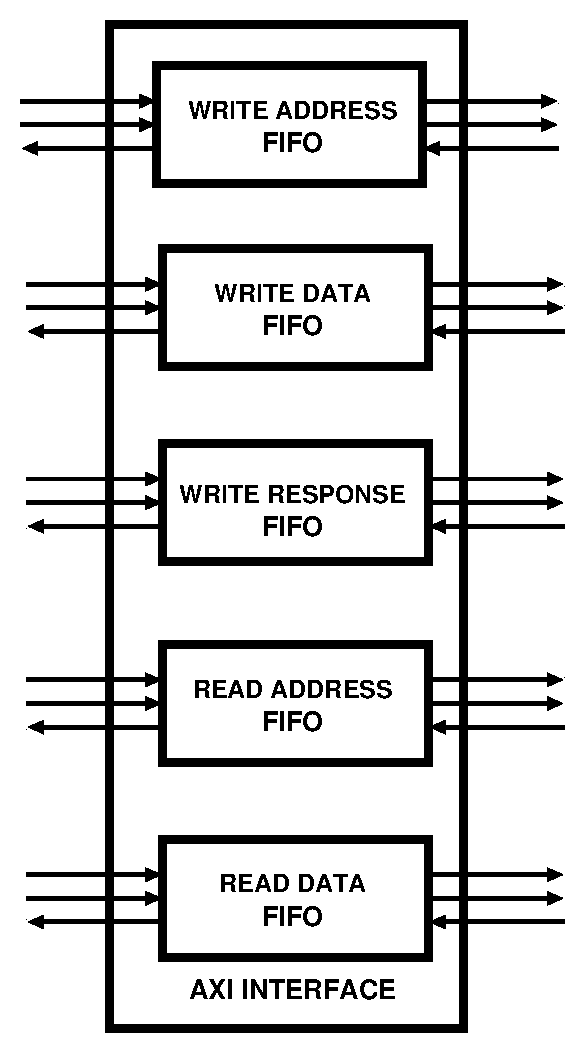
\includegraphics[width=0.7\textwidth]{eps_pdf_sources/ajit_fpga/AFB_AXI_bridge/AXI_internal_FIFOs}
	\caption{AXI-Lite FIFOs}
	\end{subfigure}
	\hfill
	\begin{subfigure}[b]{0.45\textwidth}
	\centering
	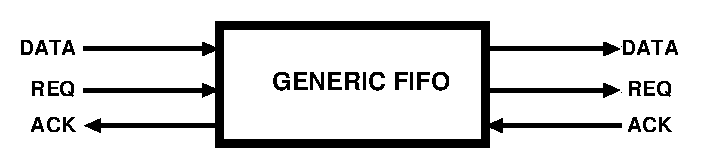
\includegraphics[width=\textwidth]{eps_pdf_sources/ajit_fpga/AFB_AXI_bridge/FIFO}
	\caption{FIFO Interface}
	\end{subfigure}
\caption{AXI-Lite Interface}
\end{figure}

\section{AFB Interface}
The master interface for the custom AFB interface is the AFB Request Interface and the corresponding slave interface is the AFB Response
Interface.

- Need to add AFB specs table.

\subsection{AFB Response Interface}
\begin{table}[H]
\begin{tabular}{c | c | c | c}	
\hline
Port Name & Port Description & Direction & VHDL Data Type\\
\hline
AFB\_RESP\_DATA 	& Data Signal 	& in & std\_logic\_vector(32 downto 0) \\
AFB\_RESP\_READY 	& Ready Signal 	& in & std\_logic\_vector(0 downto 0)  \\
AFB\_RESP\_ACCEPT & Acceptance Signal & out & std\_logic\_vector(0 downto 0)  \\
\end{tabular}
\caption{AFB Response Interface Signals}
\end{table}

\subsection{AFB Request Interface}
\begin{table}[H]
\begin{tabular}{c | c | c | c}
\hline
Port Name & Port Description & Direction & VHDL Data Type\\
\hline
AFB\_REQ\_DATA 	 & Data Signal	     & out  & std\_logic\_vector(32 downto 0) \\
AFB\_REQ\_READY  & Ready Signal      & in   & std\_logic\_vector(0 downto 0)  \\
AFB\_REQ\_ACCEPT & Acceptance Signal & out  & std\_logic\_vector(0 downto 0)  \\
\end{tabular}
\caption{AFB Response Interface Signals}
\end{table}

\section{Req and Ack Interface Protocol}
Req and Ack protocol is a custom protocol defined by Prof.Madhav Desai wherein the environment sends out a \verb|req| signal whenever it has
data to send out and the slave responds with an \verb|ack| signal which translates to a green flag to the transaction and the data is
exchanged.  The \verb|req| and \verb|ack| signals are interchangeable and thus can be asserted by the environment or by the slave.
Figure~\ref{req_ack_protocol} shows the timing diagram for the req-ack protocol:-

\begin{figure}[H]
\centering
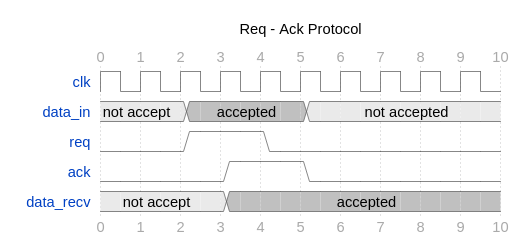
\includegraphics[width=\textwidth]{eps_pdf_sources/ajit_fpga/Interfaces/req_ack_protocol.png}
\caption{Timing diagram of Req-Ack protocol}
\label{req_ack_protocol}
\end{figure}

\section{HLS Stream Interface}
This is a trivial fifo like interface which can be generated through Vivado HLS. It uses \verb|ready| and \verb|accept| signals
instead of \verb|req| and \verb|ack|. Figure~\ref{ready_accept_protocol} shows the timing diagram for the ready-accept protocol:-

\begin{figure}[H]
\centering
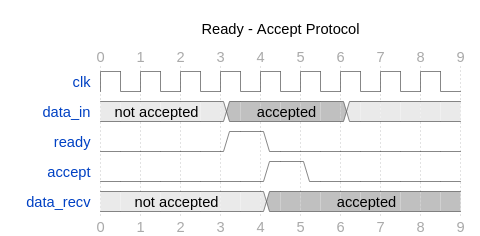
\includegraphics[width=\textwidth]{eps_pdf_sources/ajit_fpga/Interfaces/ready_accept_protocol.png}
\caption{Timing diagram of HLS stream interface}
\label{Ready-Accept protocol}
\end{figure}
